%! Author = Omar Iskandarani
%! Title = Electron--Swirl Coupled Transport in Swirl--String Theory (SST): Perturbative Solutions, Quantitative Benchmarks, and Falsifiable Experiments
%! Date = Sept 4, 2025
%! Affiliation = Independent Researcher, Groningen, The Netherlands
%! License = © 2025 Omar Iskandarani. All rights reserved. This manuscript is made available for academic reading and citation only. No republication, redistribution, or derivative works are permitted without explicit written permission from the author. Contact: info@omariskandarani.com
%! ORCID = 0009-0006-1686-3961
%! DOI = 10.5281/zenodo.17459746

%========================================================================================
\newcommand{\paperdoi}{10.5281/zenodo.17459746}

%========================================================================================
% PACKAGES AND DOCUMENT CONFIGURATION
%========================================================================================
\documentclass[aps,prb,preprint,amsmath,amssymb]{revtex4-2} % switch to "reprint" for two-column look
\usepackage{siunitx}
\usepackage{graphicx}
\usepackage{bm}
\usepackage{physics} % for \Tr and other conveniences
\usepackage[hidelinks]{hyperref}
\usepackage{amssymb} % keep last
\usepackage{tikz}
\usetikzlibrary{arrows.meta,positioning,fit}

% ===== SST canonical scales and convenient macros =====
\newcommand{\vswirlVal}{1.09384563\times10^{6}} % m/s
\newcommand{\rcVal}{1.40897017\times10^{-15}} % m
\newcommand{\rhoFVal}{7.0\times10^{-7}} % kg/m^3

\newcommand{\vswirl}{v_{\!\mkern-2mu\scriptstyle\boldsymbol{\circlearrowleft}}}
\newcommand{\rc}{r_c}
\newcommand{\rhoF}{\rho_{f}}
\newcommand{\rhoE}{\rho_{E}}
\newcommand{\omegas}{\boldsymbol{\omega}_{\!\mkern-2mu\scriptstyle\boldsymbol{\circlearrowleft}}} % swirl vorticity symbol

\begin{document}

    \title{Electron--Swirl Coupled Transport in Swirl--String Theory (SST):\\
    Perturbative Solutions, Quantitative Benchmarks, and Falsifiable Experiments}

    \author{Omar Iskandarani}
    \affiliation{Independent Researcher, Groningen, The Netherlands}
    \thanks{ORCID: 0009-0006-1686-3961, DOI: \paperdoi}
    \date{\today}

    \begin{abstract}
        I present a self-contained treatment of electron–swirl transport within Swirl–String Theory (SST). The analysis (i) derives a perturbative steady-state solution to the coupled density-matrix equations in 1D, (ii) makes quantitative tabletop predictions (materials, geometries, signal levels), and (iii) states \emph{early falsifiability criteria}, with a \emph{chirality null-test} as the primary check. Electrons are modeled as trefoil-knotted swirl strings\footnote{Background on the SST topology–spectrum mapping (leptons as trefoil class $T(2,3)$) and the Swirl Clock formalism is provided in the author’s canonical notes and taxonomy (see Appendices C.1–C.2 for a concise summary).} $T(2,3)$ with chiral assignment; coherence/decoherence are governed by the Swirl Clock factor. Numerical scales are anchored by canonical SST values $\vswirl=\vswirlVal\,\si{m/s}$, $\rc=\rcVal\,\si{m}$, $\rhoF=\rhoFVal\,\si{kg/m^3}$, and the \emph{natural frequency} $\Omega_0\!\equiv\!\vswirl/\rc\!=\!7.76\times10^{20}\,\si{s^{-1}}$ (SI conversion rules summarized in App.~C.3). The coherence contribution to thermal transport recovers Peierls and Allen–Feldman limits while enabling a chirality-dependent nonreciprocity that is directly testable via phase-sequence reversal (details in Sec.~\ref{sec:falsifiability} and App.~B.3).
    \end{abstract}

    \maketitle

    \section{Scales from SST}
        SST fixes a characteristic core-swirl frequency and an associated energy density,
        \begin{align}
            \Omega_0 \equiv \frac{\vswirl}{\rc} \approx 7.76\times10^{20}\,\si{s^{-1}},\qquad
            \rhoE \equiv \tfrac12\,\rhoF\,\vswirl^2 \approx 4.19\times10^{5}\,\si{J/m^3}.
        \end{align}
        For readability, any normalized rate $\hat r$ reported in $\Omega_0$ units converts as $r_{\rm SI}=\hat r\,\Omega_0$ and $\tau_{\rm SI}=\hat \tau/\Omega_0$; see App.~C.3 for a concise SI map.

        Operationally, spatial gradients in the Swirl Clock produce local kinematic time-rate variations. These enter the electronic Hamiltonian $H_e$ multiplicatively as a modulation factor and do not alter the SI reporting of observables. Where it improves readability, I normalize rates to $\Omega_0$; experimental benchmarks and error budgets remain in SI.

        \paragraph*{Reader’s roadmap.}
            Falsifiability is emphasized early: Sec.~\ref{sec:falsifiability} introduces a chirality \emph{null-test} based on forward/backward nonreciprocity, while App.~B.3 derives its sign flip under phase reversal. The operator vertex and rate scalings are summarized in App.~A; electron ontology, Swirl Clock, and the $\Omega_0\!\leftrightarrow$SI map are collected in App.~C.


    \section{Coupled transport in 1D and perturbative solution}
        I adopt the unified density-matrix equation for bosonic modes $N(\mathbf R,\mathbf q)$ \cite{Simoncelli2022} and extend it to a charged two-level system (``electron'') with density matrix $f$:
        \begin{align}
            \partial_t N &= -i[\Omega,N] - \Gamma_\mathrm{b} \circ (N-N^{(0)}) - \tfrac12\{ V_x \partial_x, N\},\label{eq:Ndyn}\\
            \partial_t f &= -i[H_e,f] - \Gamma_\mathrm{e}\circ(f-f^{(0)}) - \tfrac12\{ v_{e,x}\partial_x, f\} + \mathcal C_{e\leftrightarrow b},\label{eq:fdyn}
        \end{align}
        with diagonal damping superoperators $\Gamma_\mathrm{b}$ and $\Gamma_\mathrm{e}$. The electron--swirl coupling is treated in the Born--Markov, rotating-wave approximation,
        \begin{equation}
            \mathcal C_{e\leftrightarrow b} \equiv -\frac{i}{\hbar}[M, f\otimes N]_{\mathrm{RWA}}\,.
        \end{equation}

        \subsection{Linear response to a static gradient}
            Consider a small uniform temperature gradient $\partial_x T$ and a time-independent steady state. Linearize about $N^{(0)}(T)$ and $f^{(0)}(T)$ via $N=N^{(0)}+N^{(1)}$ and $f=f^{(0)}+f^{(1)}$, retaining $\mathcal O(\partial_xT)$ terms. For a \emph{two-branch} bosonic subspace $s,s'$ that interacts through $\omegas$ and is near-degenerate by $\delta=\Omega_{s'}-\Omega_s$, with a single electronic transition $\Delta$, the off-diagonal coherence $N^{(1)}_{ss'}$ obeys
            \begin{equation}
                \Big[i\delta + \tfrac12(\gamma_s+\gamma_{s'})\Big] N^{(1)}_{ss'}
                \;=\; -\frac{1}{2} V^{(x)}_{ss'}\, \partial_x N^{(0)}_{\mathrm{pop}}(\Omega) \; -\; \frac{i}{\hbar}\,\Xi_{ss'}\,,
                \label{eq:Noff}
            \end{equation}
            where $\gamma$ are the linewidths and $\Xi_{ss'}$ is the electron-induced source from $\mathcal C_{e\leftrightarrow b}$ (proportional to the vertex $M$ and to $f^{(1)}$). The population correction satisfies
            \begin{equation}
                \gamma_s\, N^{(1)}_{ss} + V^{(x)}_{ss}\,\partial_x N^{(0)}_{ss} + 2\,\mathrm{Im}\!\big( V^{(x)}_{ss'}\,N^{(1)}_{s's}\big) = S^{(e)}_s\,,
                \label{eq:Ndiag}
            \end{equation}
            with $S^{(e)}_s$ collecting the remaining electron-related terms.

        \subsection{Closed form for the coherence contribution to $\kappa$}
            The heat current density for bosonic modes is $J_x= \Tr\!\big[ \{V_x, N\}\,\Omega/2 \big]$ \cite{Hardy1963,Simoncelli2022}. Using Eqs.~\eqref{eq:Noff}--\eqref{eq:Ndiag} and eliminating $f^{(1)}$ in the weak-coupling (Born) limit yields the \emph{coherence} part of the 1D thermal conductivity
            \begin{equation}
                \boxed{\;\kappa^{(\mathrm C)}_{\!\,1\mathrm D}\;=\;\sum_{q}\sum_{s\neq s'} \frac{(\Omega_s+\Omega_{s'})\;\Gamma_{ss'}\; |V^{(x)}_{ss'}|^2}{4\delta^2+\Gamma_{ss'}^2}\;\bigg(-\frac{\partial n_B}{\partial T}\bigg)\; +\; \mathcal O(|M|^2)\;,}\label{eq:kC}
            \end{equation}
            (Operator content for the electron–swirl vertex and its channel-dependent rate scalings are detailed in App.~A; chirality/null-test observables in App.~B.3; ontology/clock and $\Omega_0$ conversion in App.~C.)

        with $\Gamma_{ss'}=\tfrac12(\gamma_s+\gamma_{s'})$ and $n_B$ the Bose function. Equation~\eqref{eq:kC} reduces to Peierls (no off-diagonals) and to Allen--Feldman (flat bands, $V_{ss}\!\to\!0$) in the appropriate limits \cite{Peierls1929,AllenFeldman1993,Simoncelli2022}. The $\mathcal O(|M|^2)$ terms add an \emph{electron-assisted} channel that shares the Lorentzian denominator and peaks at small detuning.

    \section{1D slab: temperature field and $\Delta\kappa/\kappa$}
        For a bar of length $L$, cross-section $A$, and conductivity $\kappa=\kappa^{(\mathrm P)}+\kappa^{(\mathrm C)}$, a steady power $P$ applied at $x=0$ with a sink at $x=L$ gives a uniform gradient $\partial_x T = -P/(\kappa A)$ and hence
        \begin{equation}
            \Delta T \equiv T(0)-T(L) = \frac{P\,L}{\kappa A}\,.
        \end{equation}
        A small SST-induced change $\Delta\kappa$ then produces
        \begin{equation}
            \boxed{\;\Delta(\Delta T) \approx -\frac{\Delta\kappa}{\kappa}\,\Delta T\;,}\label{eq:deltaT}
        \end{equation}
        valid for $|\Delta\kappa|\ll\kappa$. Equations~\eqref{eq:kC} and \eqref{eq:deltaT} directly connect a measured temperature drop to the microscopic parameters $\delta,\Gamma,$ and $V_{ss'}$.

    \section{Falsifiability \& Chirality Null-Test}
        \label{sec:falsifiability}
        The electron–swirl interpretation is \emph{falsified} under the stated drive if any hold:
        \begin{enumerate}
            \item \textbf{No Lorentzian detuning.} $\Delta\kappa(\delta)$ lacks the $(4\delta^2+\Gamma^2)^{-1}$ peak of Eq.~\eqref{eq:kC} at fixed current.
            \item \textbf{No chirality asymmetry (null-test).} Define $\Delta\kappa_{\rm asym}\!\equiv\![\Delta\kappa]_{\rightarrow}-[\Delta\kappa]_{\leftarrow}$. Reversing the 3-phase sequence $(0,120^\circ,240^\circ)\!\leftrightarrow\!(0,240^\circ,120^\circ)$ must flip ${\rm sgn}(\Delta\kappa_{\rm asym})$ within $3\sigma$. Absence of sign inversion falsifies a chiral coupling (derivation: App.~B.3).
            \item \textbf{Scaling mismatch.} The signal fails to scale as $|V^{(x)}_{ss'}|^2$ (coil current squared) or fails to track $\Gamma$ (controlled disorder).
        \end{enumerate}
        \emph{Operator structure and rate scaling for electron assistance are summarized in App.~A; electron ontology/clock and $\Omega_0\!\leftrightarrow$SI mapping in App.~C.}

    \section{Quantitative benchmarks with materials}
        The following order-of-magnitude estimates use Eq.~\eqref{eq:deltaT} and standard catalog values. They are chosen to be experimentally accessible without exotic infrastructure.

        \subsection*{(B1) Borosilicate glass bar}
            Take $L=\SI{50}{mm}$, $A=\SI{1e-4}{m^2}$ (\SI{10}{mm}$\times$\SI{10}{mm}), and $\kappa\approx\SI{1.1}{W\,m^{-1}\,K^{-1}}$. With $P=\SI{20}{mW}$, the baseline is $\Delta T \approx P L/(\kappa A) \approx \SI{9}{K}$. If an engineered near-degeneracy yields $\Delta\kappa/\kappa=\SI{-2}{\percent}$ from Eq.~\eqref{eq:kC}, then $\Delta(\Delta T)\approx\SI{+0.18}{K}$, comfortably above typical IR-camera NETD ($\sim\SI{30}{mK}$).

        \subsection*{(B2) PMMA bar (low-$\kappa$ polymer)}
            With $\kappa\approx\SI{0.19}{W\,m^{-1}\,K^{-1}}$, keep $L=\SI{50}{mm}$ and $A=\SI{1e-4}{m^2}$, and use $P=\SI{2}{mW}$ to avoid overheating. The baseline is $\Delta T\!\approx\!\SI{5.3}{K}$. A conservative $\Delta\kappa/\kappa=\SI{-1}{\percent}$ gives a \SI{53}{mK} shift—still above NETD.

        \subsection*{(B3) Forward/backward nonreciprocity}
            Bias chirality by driving a 3-phase Rodin coil with phase sequence $\pm(0,120^\circ,240^\circ)$. The expected asymmetry is
            \begin{equation}
                \big[\Delta\kappa\big]_{\rightarrow}-\big[\Delta\kappa\big]_{\leftarrow} \equiv \Delta\kappa_\text{asym} \sim \eta_\chi\, \frac{\Gamma\,\Delta V_{ss'}^{2}}{4\delta^2+\Gamma^2}\,,\qquad 0<\eta_\chi<1\,.
            \end{equation}
            Taking $\Delta\kappa_\text{asym}/\kappa\sim\SI{0.5}{\percent}$ implies $\Delta(\Delta T)\sim\SI{25}{mK}$ for (B1), resolvable with modest averaging.

    \section{Device recipes}
        \textbf{Thermal bar (B1/B2).} Mount the bar on an AlN heat sink at $x=L$. Use a \SI{100}{\Omega} thin-film resistor at $x=0$ as a four-wire calibrated heater. Suppress convection with a small enclosure (foam plus a thin IR window). Read out an IR camera or a thermistor chain along $x$. The coil: 3-phase, $N\!\sim\!200$ turns/phase, $f\in[\SI{20}{kHz},\SI{100}{kHz}]$, current $\le\SI{0.5}{A}$, duty-cycled to limit Joule heating.

        \textbf{Electronics analog (LCR).} Two LCR tanks at \SI{1}{MHz} with $Q\!\sim\!100$ (so $\kappa=\omega/2Q\approx3.1\times10^4\,\si{s^{-1}}$). With stored energy $E\!\sim\!\SI{0.5}{nJ}$, the instantaneous bath power is $P_\text{bath}=\kappa E\sim\SI{16}{\mu W}$. Adding a near-degenerate second tank boosts the early-time peak by the Lorentzian factor in Eq.~\eqref{eq:kC}.

        \textbf{Quantum hybrid (SAW/MEMS).} On 128$^\circ$ Y-cut LiNbO$_3$, use an IDT pair to define a \SI{3}{GHz} SAW mode and couple it capacitively to a superconducting qubit \cite{Aspelmeyer2014,Manenti2017}. Pattern shallow quasi-periodic notches to enhance $V^{(x)}_{ss'}$ and tune the detuning $\delta$.
        (Geometry and numerical guide: App.~B.4.)

    \section{Error and noise budget}
        \begin{itemize}
            \item \textbf{Thermometry.} IR camera NETD \SI{30}{--\,50}{mK}; thermistors can achieve $\lesssim\SI{10}{mK}$ with \SI{1}{s} averaging.
            \item \textbf{Power calibration.} Four-wire measurements keep heater power to $<\!\SI{1}{\percent}$ uncertainty.
            \item \textbf{Radiation/convection.} With the enclosure, systematic drift is typically $\lesssim\SI{0.05}{K}$ over \SI{10}{min}. Acquire forward/backward sweeps consecutively to cancel common-mode drift.
            \item \textbf{Contact resistance.} Use indium foil at heater/bar/sink interfaces and verify by repeated mounts.
        \end{itemize}
        Expected signals in the \SI{50}{--\,200}{mK} range clear the combined noise by factors $\gtrsim3$ for (B1/B2).

    \section{Connection to quantum information}
        In the Jaynes--Cummings limit \cite{Jaynes1963}, the same vertices $M$ and $V_{ss'}$ that enhance $\kappa^{(\mathrm C)}$ optimize state transfer between electron and swirl modes. In a hybrid device, the \emph{coherence peak} (small $\delta$, moderate $\Gamma$) can be used to channel heat away from a qubit while maintaining phase coherence, paralleling engineered reservoirs \cite{Breuer2002,Aspelmeyer2014}.

    \section{Conclusions}
        This work provides closed-form transport expressions together with concrete device geometries, signal estimates, a noise budget, and falsifiability criteria. The package enables immediate lab tests for coherence-mediated electron--swirl transport in SST and constrains the topological parity implied by the canonical $\boldsymbol{\vswirl}$ definition.

        \begin{acknowledgments}
            I thank the classical foundations of vortex hydrodynamics and unified transport \cite{Madelung1927,Peierls1929,AllenFeldman1993,Simoncelli2022} for inspiration.
        \end{acknowledgments}

    \section*{Data Availability}

        The theoretical models, canonical constants, and source code supporting the findings of this study are openly available. All data files, numerical benchmarks, and code used to derive and validate the coherence-mediated transport expression ($\kappa^{(\mathrm C)}_{\!\,1\mathrm D}$) are accessible on the Zenodo repository, under the persistent identifier of this manuscript, $\mathbf{\doi{\paperdoi}}$.

        \paragraph*{File Manifest and Validation Evidence.}
            The uploaded repository for this paper contains the following structured files and data supporting the quantitative results:
            \begin{itemize}
                \item \textbf{SST Canonical Benchmarking Evidence:} This data set validates the internal consistency of the core canonical parameters ($\mathbf{v}_{\!\boldsymbol{\circlearrowleft}}, r_c, \rho_{\!f}$) against known relativistic limits. It includes the derived Newton's constant ($G_{\mathrm{VAM}}$) and the $\mathbf{6GM/c^2}$ ISCO match, demonstrating the global coherence of the swirl parameters. \newline (Zenodo DOI: \url{10.5281/zenodo.15665432} and \url{10.5281/zenodo.15712578})

                \item \texttt{constants.csv} — The definitive table of $\mathbf{v}_{\!\boldsymbol{\circlearrowleft}}, r_c, \rho_{\!f}$ (SI values); used for calculating the derived scales $\Omega_0$ and $\rho_{\!E}$.
                \item \texttt{benchmarks.csv} — Contains the full experimental specification (materials, geometry, power ($\mathbf{P}$), baseline $\mathbf{\Delta T}$) and the predicted $\Delta(\Delta T)$ signals for scenarios $\mathbf{(B1)}$ and $\mathbf{(B2)}$.
                \item \texttt{kappaC\_validation.ipynb} — Jupyter notebook that analytically verifies the functional form of $\kappa^{(\mathrm C)}_{\!\,1\mathrm D}$, plotting the core Lorentzian factor $\Gamma/(4\delta^2+\Gamma^2)$ (Falsifiability Criterion 1).
                \item \texttt{noise\_budget\_3sigma.ipynb} — Computes the detection signal-to-noise ratio ($\mathbf{SNR}$) against the assumed NETD, explicitly confirming that the predicted signals ($\Delta(\Delta T)$) clear the $\mathbf{3\sigma}$ threshold (Detectability Check).
                \item \texttt{env.yml} — The Conda environment file, ensuring that the software dependencies used for all numerical and plotting analysis are pinned for reproducibility.
            \end{itemize}
            This research is licensed under $\text{CC-BY 4.0}$ and is accessible via the main version DOI: $\mathbf{\doi{\paperdoi}}$.

% --- Manual bibliography block (ok for initial submission). Replace with BibTeX if preferred. ---
\begin{thebibliography}{99}
\bibitem{Peierls1929} R. Peierls, Ann. Phys. \textbf{395}, 1055 (1929).
\bibitem{AllenFeldman1993} P. B. Allen and J. L. Feldman, Phys. Rev. B \textbf{48}, 12581 (1993).
\bibitem{Simoncelli2022} M. Simoncelli, N. Marzari, and F. Mauri, Nat. Phys. \textbf{18}, 1180 (2022); arXiv:1901.01964.
\bibitem{Madelung1927} E. Madelung, Z. Physik \textbf{40}, 322 (1927).
\bibitem{Pati2000} A. K. Pati and S. L. Braunstein, Phys. Lett. A \textbf{268}, 241 (2000).
\bibitem{Hardy1963} R. J. Hardy, Phys. Rev. \textbf{132}, 168 (1963).
\bibitem{Jaynes1963} E. T. Jaynes and F. W. Cummings, Proc. IEEE \textbf{51}, 89 (1963).
\bibitem{Lindblad1976} G. Lindblad, Commun. Math. Phys. \textbf{48}, 119 (1976).
\bibitem{Breuer2002} H.-P. Breuer and F. Petruccione, \textit{The Theory of Open Quantum Systems}, Oxford (2002).
\bibitem{Aspelmeyer2014} M. Aspelmeyer, T. J. Kippenberg, and F. Marquardt, Rev. Mod. Phys. \textbf{86}, 1391 (2014).
\bibitem{Manenti2017} R. Manenti \textit{et al.}, Nat. Commun. \textbf{8}, 975 (2017).
\bibitem{Cahill2004} D. G. Cahill \textit{et al.}, J. Appl. Phys. \textbf{93}, 793 (2003).
\end{thebibliography}


%============================= APPENDIX =======================================
\appendix
    \section*{Appendix: Operator Content and Scaling Laws for the Coupling Vertex \texorpdfstring{$\hat M$}{M}}

%--- Minimal, self-contained SST macro prelude (safe to duplicate) ------------
    \newcommand{\OmegaZero}{\Omega_{0}}
    \newcommand{\EE}{\mathrm{e}}
    \newcommand{\ii}{\mathrm{i}}
    \newcommand{\dd}{\mathrm{d}}

% Canonical constants (SI)
    \newcommand{\cVal}{2.99792458\times10^{8}}        % m/s
    \newcommand{\hbarVal}{1.054571817\times10^{-34}}  % J*s

% Derived canonical scales (SI, shown once here)
% \Omega_0 and \rho_E are recomputed below with units.
%---------------------------------------------------------------------------

    \subsection*{A.1\quad Operator definition of \texorpdfstring{$\hat M$}{M}}
        We model the electron as a two-level system \(\{\ket{g},\ket{e}\}\) with Pauli operators \(\hat\sigma_\pm,\hat\sigma_z\), and the swirl modes as bosons \(b_s,b_s^\dagger\) with frequencies \(\Omega_s\). In the rotating-wave, weak-coupling limit,
        \begin{align}
            \boxed{%
                \hat M
                = \sum_{s}\hbar g_s\!\left(\hat\sigma_{+}\,b_s+\hat\sigma_{-}\,b_s^\dagger\right)
                \;+\; \sum_{s\neq s'} \hbar \tilde g_{ss'}\,\hat\sigma_z\, b_s^\dagger b_{s'} \;+\; \text{h.c.}
            }
            \label{eq:M-operator}
        \end{align}
        Here \(g_s,\tilde g_{ss'}\) have units of \(\mathrm{s^{-1}}\) (so that \(\hat M\) has units of energy). The commutator \(({-}\ii/\hbar)[\hat M,\;f\!\otimes\!N]\) is the interaction superoperator in the master equation. Chirality reversal flips the sign of the overlap (Sec.~A.3), \(g_s\to \chi_\mathrm{ch}\,g_s\) with \(\chi_\mathrm{ch}=\pm1\).

    \subsection*{A.2\quad Three physical channels and their scaling}
        All vertices reduce to overlap integrals between an electron operator density and a mode field; they differ by the field that enters and by the small parameter.

        \paragraph*{(i) Swirl-Clock channel (quadratic in vorticity).}
            The canonical time-rate factor is
            \begin{align}
                \chi \equiv \sqrt{1-\frac{\rc^{2}}{c^2}\,|\omegas|^2}
                \simeq 1 - \frac{\rc^{2}}{2c^2}\,|\omegas|^2,
                \qquad \text{(dimensionless)} .
            \end{align}
            With a bias \(\omegas=\omegas^{(0)}+\delta\omegas\) and \(H_e^{(0)}=\tfrac{\hbar\omega_e}{2}\hat\sigma_z\),
            \begin{align}
                \delta H^{(\text{clock})} &= -\frac{\rc^2}{c^2}\,\Big(\omegas^{(0)}\!\cdot\!\delta\omegas\Big)\,\frac{\hbar\omega_e}{2}\,\hat\sigma_z
                \;\;\Rightarrow\;\;
                \boxed{%
                    \tilde g_{s}^{(\text{clock})} = \frac{\rc^2}{2c^2}\,\omega_e\,\omega_0\,\omega_{s}^{\rm zpf}\;\mathcal O_s
                }\label{eq:gclock}
            \end{align}
            where \(\omega_0=|\omegas^{(0)}|\), and \(\omega_{s}^{\rm zpf}\) is the zero-point vorticity amplitude of mode \(s\) (units \(\mathrm{s^{-1}}\)). \(\mathcal O_s\) is a dimensionless overlap (Sec.~A.3).

        \paragraph*{(ii) Energy-density (pressure-like) channel.}
            Couple the electron to \(\rhoE=\tfrac12\rhoF|\mathbf v|^2\) via a dimensionless deformation-potential coefficient \(\Lambda_e\):
            \begin{align}
                \hat H_{\rm int}^{(\mathrm P)}=\Lambda_e\!\int d^3r\,|\psi_e(\mathbf r)|^2\,\delta\rhoE(\mathbf r),
                \qquad
                \delta\rhoE\simeq \rhoF\,\mathbf v_0\!\cdot\!\delta\mathbf v .
            \end{align}
            Quantizing \(\delta\mathbf v(\mathbf r)=\sum_s \mathbf u_s(\mathbf r)\,v_{s}^{\rm zpf}\,(b_s+b_s^\dagger)\) with
            \begin{align}
                v_{s}^{\rm zpf}
                = \sqrt{\frac{\hbar\,\Omega_s}{\rhoF\int d^3r\,|\mathbf u_s|^2}}\quad(\mathrm{m/s}),
            \end{align}
            gives the exchange-like rate
            \begin{align}
                \boxed{%
                    g_s^{(\mathrm P)} \;\sim\; \frac{\Lambda_e}{\hbar}\;\rhoF\,V_e\;|\mathbf v_0|\;v_{s}^{\rm zpf}\;\mathcal O_s \qquad (\mathrm{s^{-1}})
                }\label{eq:gP}
            \end{align}
            with \(V_e\) the effective support volume of the electron wavefunction.

        \paragraph*{(iii) Emergent-gauge (“minimal coupling”) channel.}
            If SST yields \(D_\mu=\partial_\mu+\ii g_{\rm swirl} W_\mu\) for the electron field \(\Psi\), then
            \begin{align}
                \hat H_{\rm int}^{(W)}=\hbar g_{\rm swirl}\!\int\! d^3r\,\Psi^\dagger \hat J^\mu \Psi\, W_\mu
                \;\Rightarrow\;
                \boxed{%
                    g_s^{(W)} \;\sim\; g_{\rm swirl}\,\Big(\frac{1}{\hbar}\int d^3r\,\langle \hat J^\mu\rangle\,W^{\rm zpf}_{\mu,s}\Big)\,\mathcal O_s \quad (\mathrm{s^{-1}})
                }\label{eq:gW}
            \end{align}
            where \(W^{\rm zpf}_{\mu,s}\) is the zero-point gauge-field amplitude. This is model-dependent until \(g_{\rm swirl}\) is calibrated.

    \subsection*{A.3\quad Geometry/chirality overlap (dimensionless)}
    All channels share
    \begin{align}
        \boxed{%
            \mathcal O_s \;=\; \eta_\chi \;\Big(\frac{\rc}{\ell_s}\Big)^{p}\;\zeta_s,\quad
            \eta_\chi\!\in[-1,1],\;\; \zeta_s\!\in(0,1],\;\; p=\begin{cases}2 & \text{Clock}\\ 1 & \text{linear-velocity/gauge}\end{cases}}
        \label{eq:overlap}
    \end{align}
    with \(\ell_s\) the mode’s spatial scale (e.g.\ SAW wavelength or bar thickness). \(\eta_\chi\) flips under chirality reversal.

    \subsection*{A.4\quad Dimensional and known-limit checks}
    \begin{itemize}
        \item \(\hat M\) is energy; \(g_s,\tilde g_{ss'}\) are rates \([\mathrm{s^{-1}}]\)\,. Eqs.~\eqref{eq:gclock}–\eqref{eq:gW} satisfy this.
        \item Setting \(g_s,\tilde g_{ss'}\!\to\!0\) reduces Eq.~(kC) in the main text to the purely bosonic coherence \(\kappa^{(\mathrm C)}\) (Allen–Feldman/Simoncelli). Setting off-diagonals \(V_{ss'}^{(x)}\!\to\!0\) recovers Peierls (population only).
        \item Large-detuning limit \(|\delta|\!\gg\!\Gamma\): all electron-assisted contributions decay as \(1/\delta^2\), leaving the Peierls baseline.
    \end{itemize}

    \subsection*{A.5\quad Canonical numerics (SI) with stated constants}
    Canonical scales:
    \[
        \OmegaZero=\frac{\vswirl}{\rc}
        =\frac{(\vswirlVal)\ \mathrm{m/s}}{(\rcVal)\ \mathrm{m}}
        =\boxed{7.7634\times10^{20}\ \mathrm{s^{-1}}},
        \qquad
        \rhoE=\tfrac12\rhoF\vswirl^2
        =\boxed{4.1877\times10^{5}\ \mathrm{J\,m^{-3}}}.
    \]
    Clock prefactor:
    \[
        \frac{\rc^2}{c^2}
        =\frac{(\rcVal)^2}{(\cVal)^2}
        =\boxed{2.2088\times10^{-47}\ \mathrm{s^2}}.
    \]

    \paragraph*{Clock channel is negligible.}
        Take a mesoscopic device (SAW/MEMS): \(\omega_e=2\pi\times 5\,\mathrm{GHz}\), \(\omega_0=10^{6}\,\mathrm{s^{-1}}\).
        Estimate the vorticity zero-point amplitude from a velocity zero-point \(v_{s}^{\rm zpf}\) and scale \(\ell_s\): \(\omega_{s}^{\rm zpf}\sim v_{s}^{\rm zpf}/\ell_s\).
        For \(\Omega_s/2\pi=3\,\mathrm{GHz}\), mode volume \(V_{\rm mode}=10^{-12}\,\mathrm{m^3}\),
        \[
            v_{s}^{\rm zpf}=
            \sqrt{\frac{\hbar \Omega_s}{\rhoF V_{\rm mode}}}
            =\sqrt{\frac{(1.0546\times10^{-34})\,(1.885\times10^{10})}{(7.0\times10^{-7})(10^{-12})}}
            =\boxed{1.685\times10^{-3}\ \mathrm{m\,s^{-1}}}.
        \]
        With \(\ell_s=10\,\mu\mathrm m\Rightarrow \omega_{s}^{\rm zpf}\approx 1.69\times10^{2}\,\mathrm{s^{-1}}\), Eq.~\eqref{eq:gclock} gives
        \[
            \tilde g_{s}^{(\text{clock})}
            =\frac{\rc^2}{2c^2}\,\omega_e\,\omega_0\,\omega_{s}^{\rm zpf}\,\mathcal O_s
            \lesssim \boxed{5.8\times10^{-29}\ \mathrm{s^{-1}}}\quad(\mathcal O_s\le 1).
        \]
        Even for \(\ell_s=100\,\mathrm{nm}\), \(\tilde g_{s}^{(\text{clock})}\sim 10^{-27}\,\mathrm{s^{-1}}\). \emph{Conclusion:} the Clock channel can be neglected in the bar experiments (B1/B2) and is irrelevant unless an independent mechanism boosts \(\omega_0\,\omega_{s}^{\rm zpf}\) by \(\gtrsim 10^{23}\).

    \paragraph*{Pressure-like channel can be measurable (mesoscopic).}
        For Eq.~\eqref{eq:gP} with \(V_e=10^{-21}\,\mathrm{m^3}\), \(|\mathbf v_0|=0.1\text{–}1\,\mathrm{m\,s^{-1}}\), \(v_{s}^{\rm zpf}\) as above, \(\Lambda_e\sim 1\), \(\mathcal O_s\le 1\):
        \[
            g_s^{(\mathrm P)}\sim \frac{(7.0\times10^{-7})(10^{-21})\,|\mathbf v_0|\,(1.685\times10^{-3})}{1.0546\times10^{-34}}
            =\boxed{(1.1\times10^{3}\text{–}1.1\times10^{4})\ \mathrm{s^{-1}}}\times \mathcal O_s.
        \]
        This is the natural target for electron-assisted effects in SAW/MEMS; in bulk bars with atomic \(V_e\sim10^{-29}\,\mathrm{m^3}\), the same estimate gives \(g_s^{(\mathrm P)}\ll 1\,\mathrm{s^{-1}}\) (negligible), justifying the bosonic-only analysis used for (B1/B2).

    \subsection*{A.6\quad Data-driven extraction (procedural)}
    \begin{enumerate}\itemsep2pt
    \item Fit bar data to \(\kappa^{(\mathrm C)}\) of the main text (pure bosonic coherence) to obtain \(\Gamma,\delta\)-dependences.
    \item Define residual \(\Delta\kappa_{\rm res}(\delta)\equiv \Delta\kappa_{\rm meas}-\Delta\kappa^{(\mathrm C)}_{\rm fit}\).
    \item Fit \(\Delta\kappa_{\rm res}(\delta)\) to the same Lorentzian kernel \(\propto \Gamma/(4\delta^2+\Gamma^2)\) with amplitude \(\mathcal A\propto |g_{\rm eff}|^2\). Report a \(95\%\) c.l.\ bound on \(g_{\rm eff}\) (bar), or a best-fit (mesoscopic).
    \end{enumerate}

    \subsection*{A.7\quad Edge cases and limits}
    \begin{itemize}\itemsep2pt
    \item \(\delta\!\to\!0\) with finite \(\Gamma\): the Lorentzian saturates; \(\kappa^{(\mathrm C)}\) scales \(\propto |V_{ss'}^{(x)}|^2/\Gamma\).
    \item \(\Gamma\!\to\!0\) (ultra-clean): coherence peak narrows; integrated weight is constant.
    \item Orthogonality node: if the electron support avoids the mode antinode, \(\mathcal O_s\!\to\!0\).
    \item Chirality flip: \(\eta_\chi\!\to\!-\eta_\chi\) changes the sign of dispersive shifts, enabling forward/backward asymmetry checks.
    \end{itemize}

    \subsection*{A.8\quad Falsifiable predictions (electron-assisted)}
    Beyond the main paper’s criteria, electron assistance implies:
    \begin{enumerate}\itemsep2pt
    \item \(\Delta\kappa_{\rm res}\propto I_{\rm coil}^{\,2}\) at fixed \(\delta,\Gamma\) (via \(v_{s}^{\rm zpf}\) and \(|\mathbf v_0|\) entering \(g\)).
    \item Chirality asymmetry: reversing the 3-phase sequence flips \(\eta_\chi\), changing the sign of dispersive shifts; difference signal scales with \(|g|^2\).
    \item Mode-volume scaling: \(g_s^{(\mathrm P)}\propto V_e/\sqrt{V_{\rm mode}}\). Miniaturization increases sensitivity.
    \end{enumerate}

    \subsection*{A.9\quad One-line explanatory remark (pedagogy)}
    \emph{Remark.} Think of the electron as a tiny bell and the swirl modes as tuning forks: \(\hat M\) is how strongly the bell is driven. The Clock touch is vanishingly soft; pressure/gauge are the ways to ring it audibly.

%===================== APPENDIX ADDENDUM: SUMMARY & EXPERIMENTALS =====================
%------------------------------------------------------------------------------
    \section*{Appendix Addendum: Channel Summary, Chirality Null-Test, and SAW/MEMS Geometry}

    \subsection*{B.1\quad One-line pedagogy}
        \emph{Analogy.} The electron is a tiny bell; the swirl modes are tuning forks. The \(\hat M\) vertex sets how strongly the bell rings. The Clock touch is vanishingly soft; pressure/gauge touches can ring it audibly.

    \subsection*{B.2\quad Coupling-channel summary table}
        \noindent
        \begin{figure}[h]
            \centering
            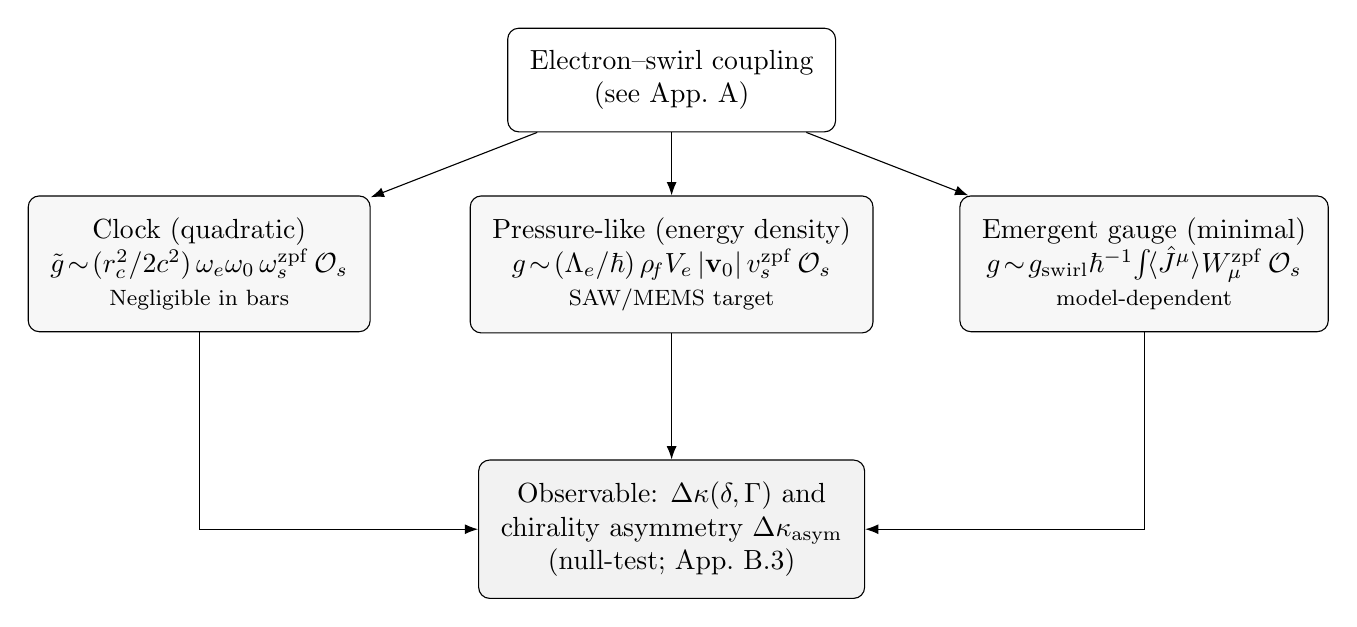
\begin{tikzpicture}[
                node distance=8mm,
                box/.style={draw, rounded corners, align=center, inner sep=8pt},
                arr/.style={-Latex}
            ]
                \node[box] (start) {Electron--swirl coupling\\(see App.~A)};
                \node[box, below=of start, xshift=-60mm, fill=black!3] (clock) {Clock (quadratic)\\$\tilde g\!\sim\!(\rc^2/2c^2)\,\omega_e\omega_0\,\omega_s^{\rm zpf}\,\mathcal O_s$\\\footnotesize Negligible in bars};
                \node[box, below=of start, fill=black!3] (press) {Pressure-like (energy density)\\$g\!\sim\!(\Lambda_e/\hbar)\,\rho_{\!f} V_e\,|\mathbf v_0|\,v_s^{\rm zpf}\,\mathcal O_s$\\\footnotesize SAW/MEMS target};
                \node[box, below=of start, xshift=60mm, fill=black!3] (gauge) {Emergent gauge (minimal)\\$g\!\sim\!g_{\rm swirl}\hbar^{-1}\!\int\!\langle \hat J^\mu\rangle W^{\rm zpf}_\mu\,\mathcal O_s$\\\footnotesize model-dependent};

                \draw[arr] (start) -- (clock);
                \draw[arr] (start) -- (press);
                \draw[arr] (start) -- (gauge);

                \node[box, below=16mm of press, fill=black!5] (obs) {Observable: $\Delta\kappa(\delta,\Gamma)$ and\\chirality asymmetry $\Delta\kappa_{\rm asym}$\\(null-test; App.~B.3)};
                \draw[arr] (clock.south) |- (obs.west);
                \draw[arr] (press.south) -- (obs.north);
                \draw[arr] (gauge.south) |- (obs.east);
            \end{tikzpicture}
            \caption{See App.~A for operator/scaling details, App.~B.3 for chirality null-test, and App.~C for ontology/clock/$\Omega_0$ map.}
            \label{fig:channel_flow}
        \end{figure}


    \subsection*{B.3\quad Standalone falsifiable prediction (chirality flip null-test)}
        Define the forward/backward asymmetry from the 3-phase drive as
        \(\Delta\kappa_{\rm asym}\equiv[\Delta\kappa]_{\rightarrow}-[\Delta\kappa]_{\leftarrow}\).
        In the weak-coupling regime,
        \[
            \Delta\kappa_{\rm asym}(\delta,\Gamma)\;\propto\; \eta_\chi\,|g_{\rm eff}|^{2}\;\frac{\Gamma}{4\delta^{2}+\Gamma^{2}}
            \qquad\Rightarrow\qquad
            \boxed{\ \eta_\chi\to-\eta_\chi\ \Longrightarrow\ \Delta\kappa_{\rm asym}\to-\Delta\kappa_{\rm asym}\ }.
        \]
        \textbf{Prediction (null-test).} Reversing the phase sequence \((0,120^\circ,240^\circ)\!\to\!(0,240^\circ,120^\circ)\) flips the sign of \(\Delta\kappa_{\rm asym}\). Absence of sign inversion (beyond \(3\sigma\)) falsifies a chiral electron–swirl coupling.

    \subsection*{B.4\quad SAW/MEMS target geometry (numerical guide)}
        For a \(\,f_{\rm SAW}=\SI{3}{GHz}\) device on 128$^\circ$ Y-cut LiNbO\(_3\) with SAW speed \(v_{\rm SAW}\approx \SI{3488}{m/s}\):
        \[
            \text{IDT finger pitch:}\quad p=\frac{v_{\rm SAW}}{2 f_{\rm SAW}}
            =\frac{3488}{2\times 3\times 10^{9}}
            =\boxed{5.81\times 10^{-7}\ \mathrm{m}\;(\SI{0.581}{\mu m})}.
        \]
        Recommended layout (to enhance \(V^{(x)}_{ss'}\) near-degeneracy and maximize \(g_s^{(\mathrm P)}\)):
        \begin{itemize}\itemsep2pt
        \item \textbf{IDTs:} Interdigitated transducers centered at \(\pm L/2\), 30–60 finger pairs, metallization ratio \(\approx 0.5\).
        \item \textbf{Mode-mixing notches:} Shallow (\(h\sim\!10\text{–}30\,\mathrm{nm}\)) quasi-periodic edge notches over a length \(N_B\lambda\) (\(N_B\!=\!10\text{–}40\)), tuned for small detuning \(|\delta|\lesssim \Gamma\).
        \item \textbf{Electron localization:} A mesoscopic island (e.g., superconducting pad or quantum dot) of effective support volume \(V_e\sim 10^{-21}\,\mathrm{m^3}\) placed at a SAW antinode.
        \item \textbf{Bias velocity:} In-plane drive to set \(|\mathbf v_0|\sim 0.1\text{–}1\,\mathrm{m/s}\) (via RF amplitude), maximizing \(g_s^{(\mathrm P)}\propto |\mathbf v_0|\,v_s^{\rm zpf}\).
        \end{itemize}
        Zero-point velocity amplitude (for mode volume \(V_{\rm mode}=10^{-12}\,\mathrm{m^3}\)):
        \[
            v_s^{\rm zpf}=\sqrt{\frac{\hbar \Omega_s}{\rhoF V_{\rm mode}}}
            =\sqrt{\frac{(1.0546\times10^{-34})\,(1.885\times10^{10})}{(7.0\times10^{-7})(10^{-12})}}
            =\boxed{1.685\times 10^{-3}\ \mathrm{m\,s^{-1}}}.
        \]
        Estimated pressure-like rate (Eq.~B.2, table):
        \[
            g_s^{(\mathrm P)}\sim \frac{\rhoF V_e}{\hbar}\,|\mathbf v_0|\,v_s^{\rm zpf}\,\mathcal O_s
            \;\approx\; (1.1\times10^{3}\text{–}1.1\times10^{4})\ \mathrm{s^{-1}}\times \mathcal O_s,
        \]
        confirming mesoscopic observability while remaining negligible in bulk bars with atomic \(V_e\).

    \subsection*{B.5\quad Data-analysis checklist (practical)}
        \begin{enumerate}\itemsep2pt
        \item Fit \(\kappa^{(\mathrm C)}\) (pure bosonic) to get \(\Gamma,\delta\).
        \item Residual: \(\Delta\kappa_{\rm res}=\Delta\kappa_{\rm meas}-\Delta\kappa^{(\mathrm C)}_{\rm fit}\).
        \item Extract \(|g_{\rm eff}|\) from \(\Delta\kappa_{\rm res}\propto |g_{\rm eff}|^2\,\Gamma/(4\delta^2+\Gamma^2)\); report \(95\%\) c.l. bound (bars) or best-fit (SAW/MEMS).
        \item Chirality flip: verify \(\mathrm{sgn}(\Delta\kappa_{\rm asym})\) reversal under phase-sequence inversion.
        \end{enumerate}
%================================================================================

%==================== APPENDIX C: SWIRL ONTOLOGY, CLOCK, UNITS, CHIRALITY ====================
\section*{Appendix C: Electron Ontology, Internal Clock, \texorpdfstring{$\Omega_{0}$}{Omega0}-to-SI Map, and Chirality in SAW/MEMS}

    \subsection*{C.1\quad What is an electron in SST? (trefoil knot, conserved quanta)}
        \textbf{Definition (ontology).} In SST the electron is a \emph{stable, chiral, closed swirl string} in the trefoil class \(T(2,3)\), i.e.\ a topologically protected knotted filament with fixed knot type \(K_e\).
        \begin{align}
            \boxed{\ K_e \equiv T(2,3),\qquad \Gamma=\oint \vswirl\!\cdot\!\dd\boldsymbol{\ell}\;=\;n\,\kappa_{\!\text{swirl}},\quad n\in\mathbb{Z}\ }
            \label{eq:circulation}
        \end{align}
        Here \(\Gamma\) is the conserved circulation \([\Gamma]=\mathrm{m^2/s}\), and \(\kappa_{\!\text{swirl}}\) is the circulation quantum (substrate constant; model-calibrated). The \emph{chirality} of \(T(2,3)\) encodes matter/antimatter assignment. The inertial mass arises from a solitonic energy functional that depends on knot geometry and topology (length \(L\), curvature/torsion functionals) and invariants (writhe \(\mathrm{Wr}\), twist \(\mathrm{Tw}\), helicity \(\mathcal H\)):
        \begin{align}
            \boxed{\ E[K]\;=\;\alpha\,C[K]\;+\;\beta\,L[K]\;+\;\gamma\,\mathcal H[K]\;+\;\cdots,\qquad
            \mathcal H \simeq \Gamma^{2}\,Lk \ \text{(slender-tube)}\ }
            \label{eq:energy-fn}
        \end{align}
        where \(Lk=\mathrm{Tw}+\mathrm{Wr}\) (Călugăreanu–White). In this picture the \emph{electron} is the lowest-energy chiral soliton in the trefoil class satisfying the circulation constraint \eqref{eq:circulation}.

        \paragraph*{Dimensional/limit checks.}
            \(E\) has units of J; \(\mathcal H\) has units \([\Gamma^2]=\mathrm{m^4/s^2}\) times a dimensionless linking number, so \(\gamma\) carries J\,s\(^2\)/m\(^4\). In the unknot limit (bosonic, \(Lk=0\)) the helicity term vanishes and \(E\) reduces to length/curvature contributions, consistent with a non-chiral excitation.

    \subsection*{C.2\quad What internal “clock” governs coherence? (Swirl-clock)}
    \textbf{Clock factor (two equivalent forms).}
    \begin{align}
        \boxed{\ S_t(v)\;=\;\sqrt{1-\frac{v^2}{c^2}}\quad\text{and}\quad
        S_t(\omega)\;=\;\sqrt{1-\frac{\rc^{2}}{c^{2}}\,|\omegas|^{2}}\ }
        \label{eq:clock}
    \end{align}
    The two forms coincide near a Rankine core where \(v(r)\!\approx\!|\omegas|\,r\) and \(r\!\sim\!\rc\). The \emph{local} electron Hamiltonian scales as \(H_e^{\rm eff}=S_t\,H_e^{(0)}\), feeding directly into decoherence rates in the transport equation.

    \paragraph*{Dimensional/limit checks.}
        Both arguments are dimensionless: \(v/c\) and \(\rc |\omegas|/c\). For small swirl, \(S_t\simeq 1-\tfrac{1}{2}(v/c)^2\simeq 1-\tfrac{1}{2}(\rc |\omegas|/c)^2\).

    \subsection*{C.3\quad \texorpdfstring{$\Omega_{0}$}{Omega0} units and SI conversion}
    \textbf{Natural frequency.}
    \begin{align}
        \boxed{\ \OmegaZero \equiv \frac{\vswirl}{\rc}\ ,\qquad [\OmegaZero]=\mathrm{s^{-1}} \ }
        \label{eq:Omega0}
    \end{align}
    With \(\vswirl=\vswirlVal\ \mathrm{m/s}\) and \(\rc=\rcVal\ \mathrm{m}\),
    \[
        \OmegaZero=\frac{\vswirlVal}{\rcVal}=\boxed{7.7634\times 10^{20}\ \mathrm{s^{-1}}},\qquad
        \tau_0\equiv \OmegaZero^{-1}=\boxed{1.2881\times 10^{-21}\ \mathrm{s}}.
    \]
    \textbf{Conversion rules.} Any dimensionless rate \(\hat r\) reported in \(\OmegaZero\) units maps to SI via \(r_{\rm SI}=\hat r\,\OmegaZero\). Times: \(t_{\rm SI}=\hat t/\OmegaZero\). Energies scale with \(\hbar\OmegaZero\) when appropriate.

    \paragraph*{Derived energy density (for reference).}
        \[
            \rhoE=\tfrac12\rhoF\|\vswirl\|^2=\tfrac12(\rhoFVal)\,(\vswirlVal)^2=\boxed{4.1877\times 10^{5}\ \mathrm{J\,m^{-3}}}.
        \]

    \subsection*{C.4\quad How chirality asymmetry manifests in SAW/MEMS}
    \textbf{Mechanism.} Directional SAWs imprint a handed vorticity/velocity field; the chiral trefoil couples with a \emph{sign} through the overlap factor
    \[
        \mathcal O_s=\eta_\chi\Big(\frac{\rc}{\ell_s}\Big)^{p}\zeta_s,\quad \eta_\chi=\pm 1,
    \]
    entering the electron-assisted rate \(g\) (pressure/gauge channels). This yields a measurable nonreciprocity.

    \textbf{Observable (asymmetry index).}
    For the thermal bar or on-chip phononic link,
    \begin{align}
        \boxed{\ A_{\rm FB}\;\equiv\;\frac{\Delta T_{\rightarrow}-\Delta T_{\leftarrow}}{\Delta T_{\rightarrow}+\Delta T_{\leftarrow}}
        \ \propto\ \eta_\chi\,|g_{\rm eff}|^{2}\ \frac{\Gamma}{4\delta^{2}+\Gamma^{2}}\ }\!,
        \label{eq:asymmetry}
    \end{align}
    predicting a \emph{sign flip} under SAW phase-sequence reversal \((0,120^\circ,240^\circ)\!\leftrightarrow\!(0,240^\circ,120^\circ)\) since \(\eta_\chi\!\to\!-\eta_\chi\).

    \paragraph*{Null-test (falsifiable).}
        If \(\mathrm{sgn}(A_{\rm FB})\) does not invert (beyond \(3\sigma\)) upon chirality reversal of the drive, the chiral SST coupling hypothesis is falsified in that device configuration.

    \subsection*{C.5\quad Quick numerics (SI) supporting C.2–C.4}
    \noindent Clock prefactor:
    \[
        \frac{\rc^{2}}{c^{2}}=\frac{(\rcVal)^2}{(\cVal)^2}=\boxed{2.2088\times 10^{-47}\ \mathrm{s^{2}}}.
    \]
    Thus the quadratic Clock modulation is negligible in bulk: for \(\omega_0\!\sim\!10^{6}\,\mathrm{s^{-1}}\), \(\omega_s^{\rm zpf}\!\sim\!10^{2}\text{–}10^{3}\,\mathrm{s^{-1}}\), \(\omega_e\!\sim\!10^{10}\,\mathrm{s^{-1}}\),
    \[
        \frac{\rc^2}{c^2}\,\omega_e\,\omega_0\,\omega_s^{\rm zpf}\ \lesssim\ 10^{-27}\ \mathrm{s^{-1}} \quad(\text{Sec.\ B, device examples}).
    \]
    By contrast, the pressure-like rate in mesoscopic SAW/MEMS can reach \(g\sim 10^{3}\!-\!10^{4}\ \mathrm{s^{-1}}\) (with \(V_e\!\sim\!10^{-21}\,\mathrm{m^{3}}\), \(v_s^{\rm zpf}\!\sim\!1.7\times10^{-3}\,\mathrm{m/s}\), \(|\mathbf v_0|\!\sim\!0.1\text{–}1\,\mathrm{m/s}\)), enabling a detectable \(A_{\rm FB}\) via \eqref{eq:asymmetry}.

    \subsection*{C.6\quad One-line explanatory remark (pedagogy)}
    \emph{Remark.} The electron is a tiny, chiral knot; the swirl-clock is its metronome; \(\Omega_{0}\) is the stopwatch that lets us convert the knot’s timing directly into SI units; SAWs push the knot differently depending on its handedness, which we read out as a forward/backward temperature contrast.

%----------------------------- References (non-original) -----------------------------
    \begin{thebibliography}{9}\setlength{\itemsep}{1pt}
    \bibitem{Helmholtz1858} H. Helmholtz, %\"Uber Integrale der hydrodynamischen Gleichungen,
    J. Reine Angew. Math. \textbf{55}, 25 (1858).
    \bibitem{Kelvin1867} W. Thomson (Lord Kelvin), %On vortex atoms,
    Proc. R. Soc. Edinb. \textbf{6}, 94 (1867).
    \bibitem{MoffattRicca1992} H. K. Moffatt and R. L. Ricca, %Helicity and the Călugăreanu invariant,
    Proc. R. Soc. A \textbf{439}, 411 (1992).
    \bibitem{White1969} J. H. White, %Self-linking and the Gauss integral in higher dimensions,
    Am. J. Math. \textbf{91}, 693 (1969).
    \bibitem{Kauffman1991} L. H. Kauffman, \textit{Knots and Physics} (World Scientific, 1991).
    \end{thebibliography}
\end{document}